\chapter{The ATLAS experiment at the LHC}\label{chap:LHCandATLAS}
\minitoc
To probe QCD in its high-energy regime, large machines accelerating particles have to be built. In this section an overview of the experimental setup used to collect a data for this analysis will be given. The first section introduces a Large Hadron Collider (LHC). In the second section, the \atlas detector will be described. In the last section, the procedure of luminosity measurement is given

\section{The LHC accelerator complex}\label{sec:LHC}

The LHC is currently the largest accelerator in the world. It is built near Geneva, Switzerland and started its operation with the first collisions in 2009. It is located in a tunnel 27 kilometers in circumference. It can be operated with proton and lead-ion beams with energies up to 7 TeV for proton beam. It was designed to make precise studies of the Standard Model (SM) predictions and to search for a new physics beyond the SM. The heavy-ion program serves a purpose of studying nuclear matter properties and a quark-gluon plasma\cite{HILHC}.

Beams are accelerated in several stages\cite{LHCMachine}, as it is shown in Fig.~\ref{fig:LHC}. The beam source is a hydrogen gas or lead in the case of the heavy ion runs.  An electrical current is used to remove the electrons from each atom, and then the ion begins its ride through the linear accelerator. For example, proton beams are accelerated in the linear accelerator LINAC2 up to the energies of 50 MeV. Then, they are injected in the PS booster, where they are further accelerated to 1.4 GeV.  The last steps before injecting beams to the LHC are the rings of the Proton Synchrotron (PS) and Super Proton Synchrotron (SPC) that accelerate protons to 25 GeV and 450 GeV respectively. The bunch structure of the beam is formed in PS, and has a nominal pattern of 39 groups of 72 bunches with 25--50 ns time spacing. Because of a large number of protons in each bunch ($\sim 1\cdot 10^{11}$), the additional multiple interactions in collisions can happen. This is one of the processes contributing to the so-called pileup.

In the LHC ring, proton beams are accelerated up to 7 TeV (yet 6.5 TeV achieved). The beams circulate in the opposite directions inside 2 beam pipe. In order to bend beam trajectory, the pipes are surrounded by 1232 superconducting dipole magnets. The superconducting cavities are used to accelerate the protons and maintain the beam constant energy during the operation time. 

As most of the circular colliders, LHC has several experiments installed in the regions, where beams are intersecting. The main experiments are:
\begin{description}
\item [ALICE] A large Ion Collider Experiment\cite{ALICE} - a dedicated detector to study heavy-ion physics, physics of strongly interacting matter, where a new phase of matter (quark-gluon plasma) is expected;
\item [ATLAS] A Toroidal LHC ApparatuS\cite{ATLASDetectorPlot} is a largest particle detector at the LHC. It is a general purpose detector, that is used to study SM processes and searches for a new physics. A detailed description of this detector is given in Sec.~\ref{sec:ATLAS};
\item [CMS] the Compact Muon Solenoid\cite{CMS} is an another multiple purpose detector at the LHC. It is built using slightly different technologies compared to ATLAS;
\item [LHCb] the Large Hadron Collider beauty \cite{LHCb} specializes for measurement of heavy (charm and bottom) quark properties, that allow studying the mechanism of CP violation.
\end{description}


\begin{figure}[!tb]
\center{
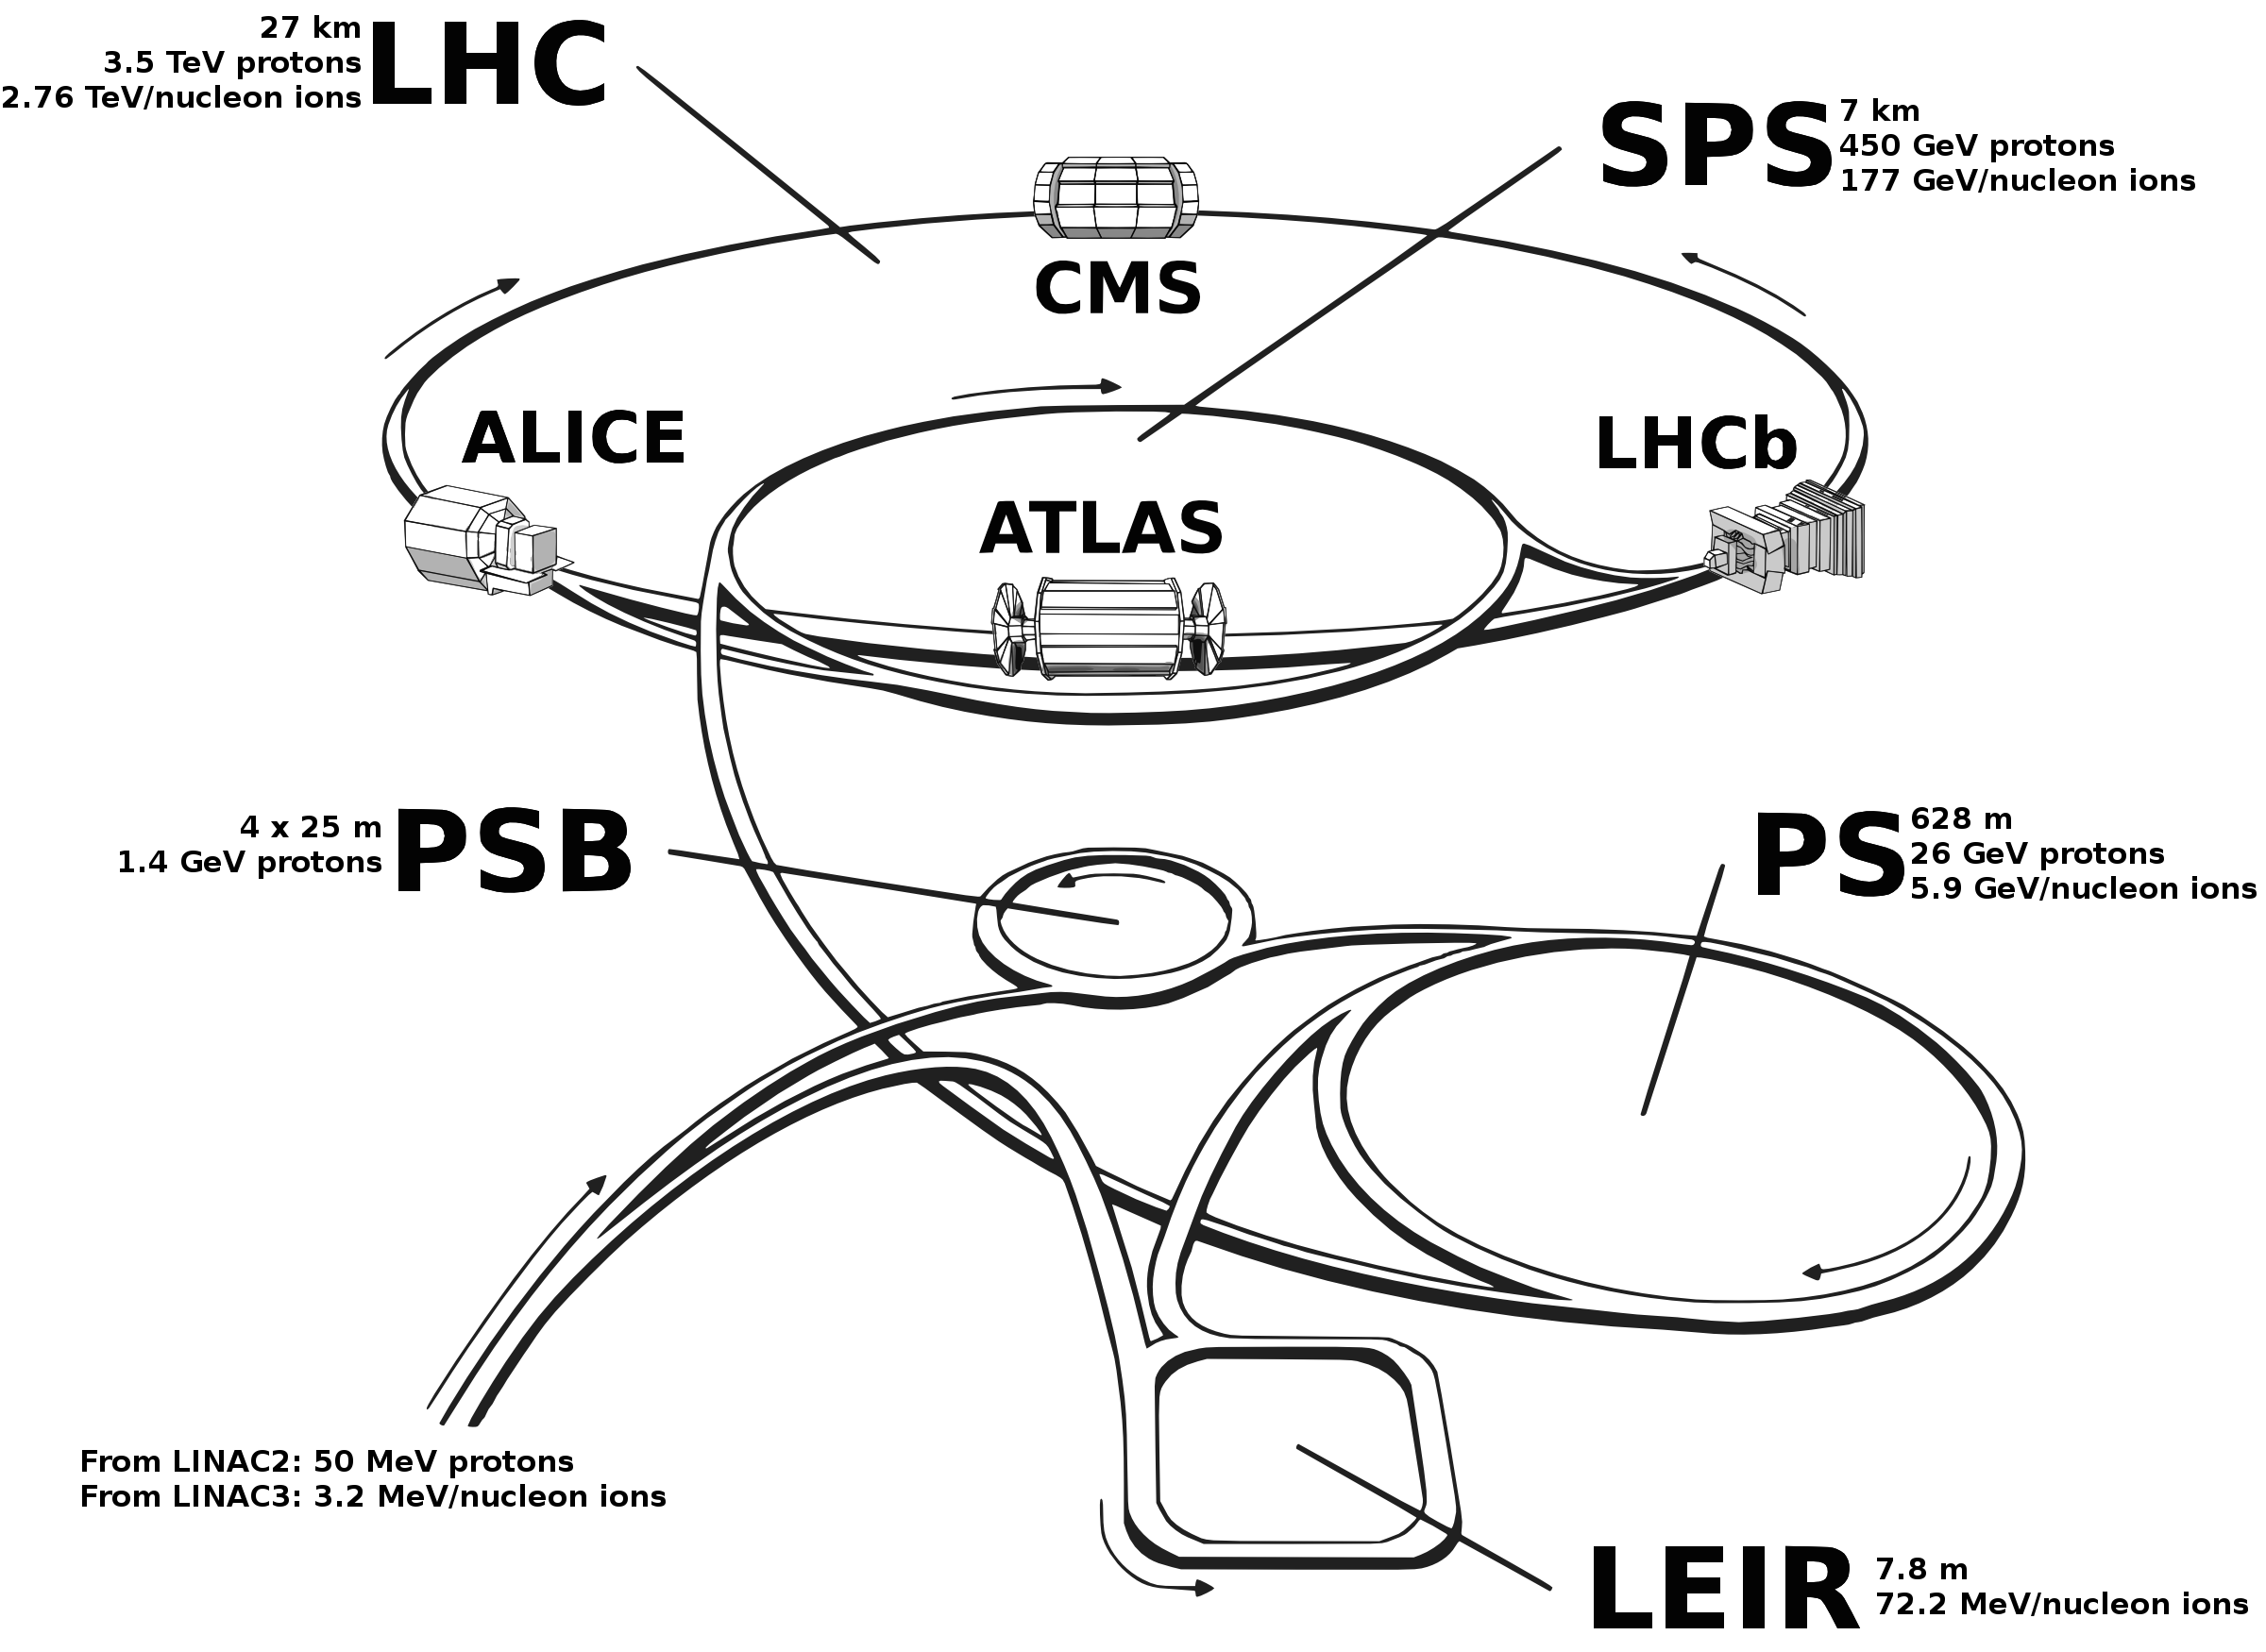
\includegraphics[width=0.7\textwidth]{LHCAtlas/cernAcceleratorComplex.png}
\caption{The LHC acceleration complex \cite{JetGoodson}.}
\label{fig:LHC}}
\end{figure}

\section{The ATLAS experiment} \label{sec:ATLAS}

\begin{figure}[!tbp]
\center{
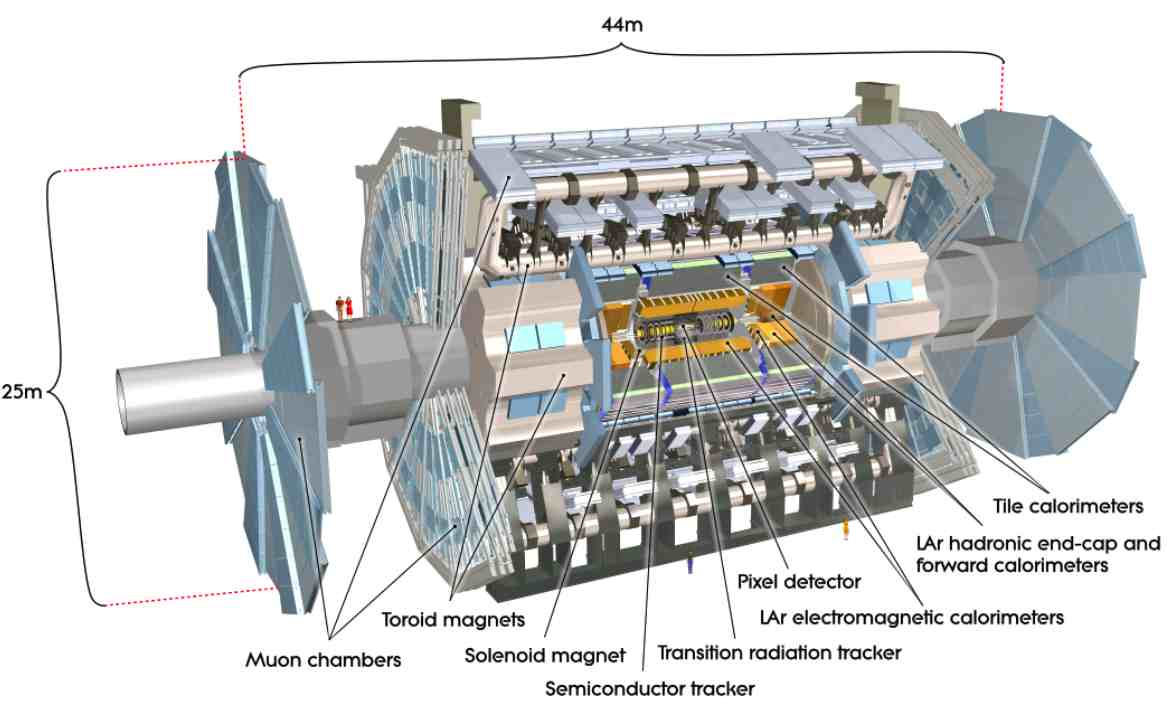
\includegraphics[width=1.0\textwidth]{LHCAtlas/ATLASDetector.png}
\caption{The ATLAS detector \cite{ATLASDetectorPlot}.}
\label{fig:ATLASDet}}
\end{figure}
The \atlas detector is a multipurpose particle detector, designed to preform various types of analysis. The schematic representation of the \atlas detector is shown in Fig.~\ref{fig:ATLASDet}. The physics goals put a strict set of requirements on the \atlas detector. Heavy particles, produced in pp collisions are expected to decay almost immediately. Thus their properties are measured only indirectly through their decay products, that should be precisely detected and identified. Good identification efficiency of photons, electrons and hadrons is achieved thanks to the system of calorimeters. Muons penetrate behind the calorimeter system, so in order to detect them, a muon chambers are built. Neutrinos escape the detector without interactions and therefore can be detected only indirectly through the energy imbalance in the detector.

The \atlas detector can be divided into 3 main subdetectors:
\begin{itemize}
\item The Inner Detector (ID), that is used for tracking and precise measurement of charged particle momentum;
\item The Calorimetry system that is used to measure the properties of electrons, photons and hadrons;
\item The muon system, designed to detect muons and measure their momenta.
\end{itemize}

Due to the symmetric LHC beams, the detector is built symmetrically around the beam pipe. The magnet system is used for tracking of charged particles for measurements of momentum and charge. The \atlas detector has 2 sets superconducting magnets: solenoid, build around the Inner Detector and toroid used together with the muon spectrometer. The strength of the magnetic field varies from 0.8 T up to 3.8 T.

\subsection{Coordinates and kinematic variables}
The detector shape motivates the choice of the coordinate system. It is natural to choose $z$ axis to be aligned with the beam, with the start in interaction point, while leaving $x$ and $y$ axis to be perpendicular to it. Because of detector symmetry along the beam $z$ axis, the cylindrical coordinates are often used, with the radial distance $r=\sqrt{x^2+y^2}$ and the polar $\theta$ and azimuth $\phi$ angles.  

The polar direction of the particles can be quantified via rapidity:
\begin{equation}
y = ln \sqrt{\frac{E+P_z}{E-P_z}},
\end{equation}
where $E$ is the energy of the particle and $P_{z}$ is the $z$ component of its momentum. In the limit of the vanishing mass, this quantity converges into another commonly used variable, called pseudorapidity:
\begin{equation}
\eta = - ln \Big[tan\Big(\frac{\theta}{2}\Big)\Big].
\end{equation}
It is preferred over the polar angle, because the difference in pseudorapidity is a Lorentz invariant under the boost in the beam direction. 

The spacial distance between two Lorentz vectors is defined as:
\begin{equation}
\Delta R = \sqrt{(\Delta\eta)^2+(\Delta\phi)^2}.
\end{equation}

Finally, the transverse momentum is defined as:
\begin{equation}
P_T=\sqrt{P_x^2+P_y^2},
\end{equation}
where $P_x$ and $P_y$ are the $x$ and $y$ components of a particle momentum respectively. Since the incoming protons are aligned along the $z$-axis and have the same energy, the total transverse momentum of all particles produced in the interaction is expected to be zero. 

\subsection{Inner Detector}

\begin{figure}[!tbp]
\center{
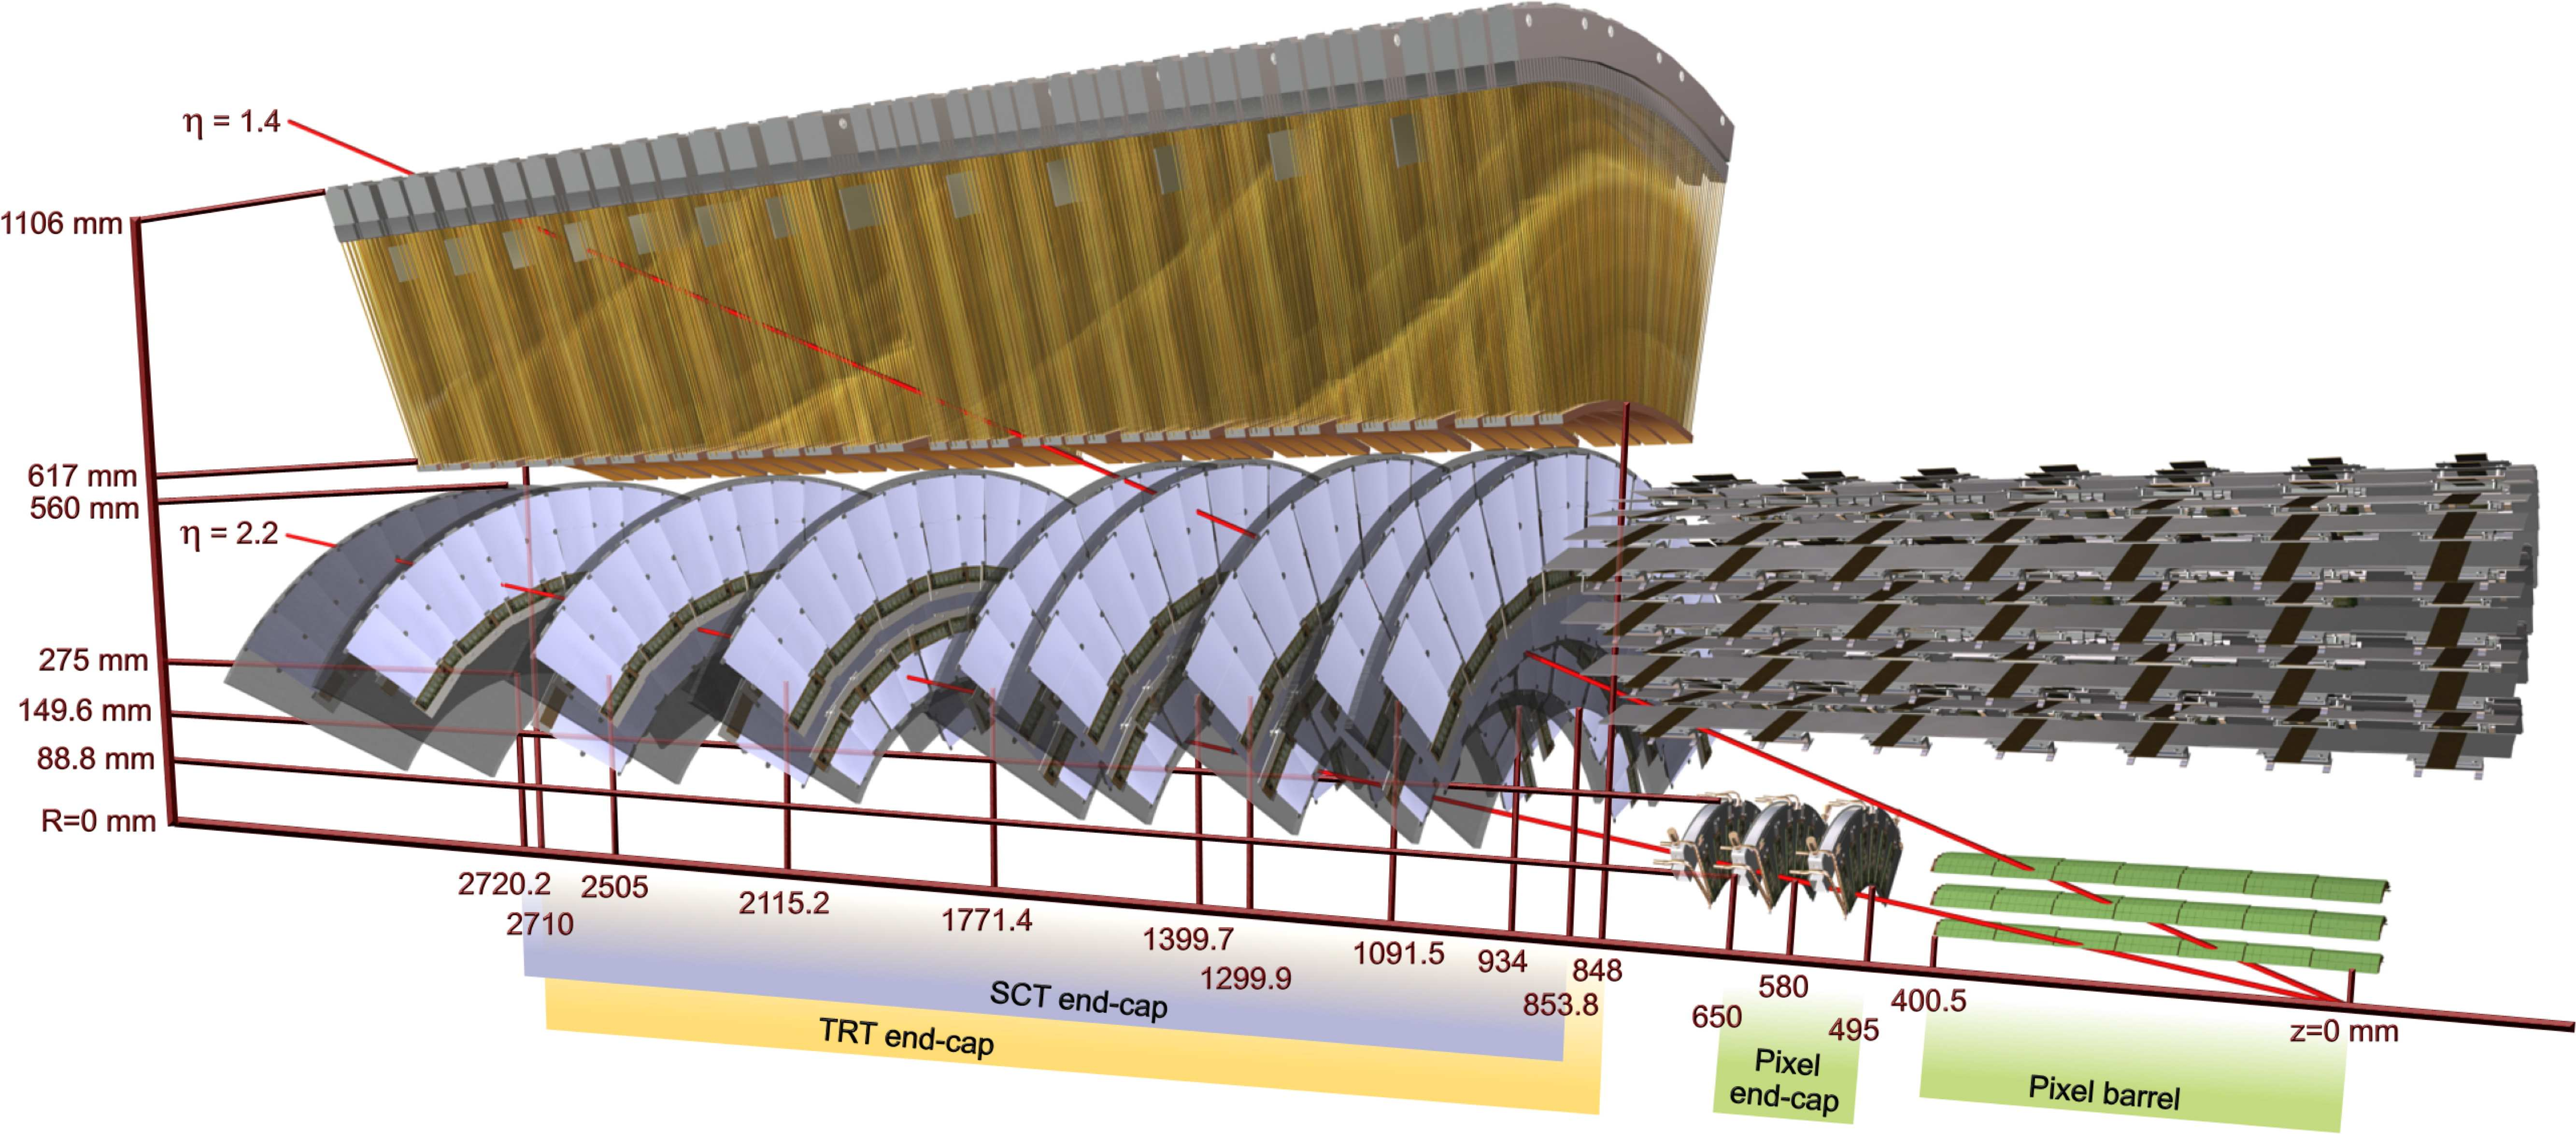
\includegraphics[width=1.0\textwidth]{LHCAtlas/FigID.pdf}
\caption{Cut-away view of the ATLAS Inner Detector. Drawing is showing the sensors and structural elements traversed by two charged with $P_T$ of 10GeV\cite{AtlasExperiment}.}
\label{fig:ATLASID}}
\end{figure}

The Inner Detector (ID) is tracking detector system being placed closest to the interaction point. It is used for reconstruction of charged particles trajectories. In order to achieve a good position resolution, it is necessary to use a high granularity detector. The layout of the ID is shown in Fig.~\ref{fig:ATLASID}. 

The ID consists of 3 sub-detectors:
\begin{itemize}
\item The pixel detector consists of approximately 80.4 million readout channels placed in 3 barrel and 3 disk layers at the end of each barrel region. Each pixel module is made of the silicon active and a layer of front-end electronics. A charged particle, passing through the module, creates electron-hole pairs, that cause a signal in the readout electronics. Pixel detector is placed close to the interaction point, which allows achieving 10 $\mu$m resolution for vertices;
\item The silicon strip detector (SCT) consists of 6.3 million readout channels. It gives a significant contribution to the measurement of charged particle momentum, because of a large number of hits the particle produces in this detector. It works in a similar way as the pixel detector, however  with the  smaller tracking precision. On average, each track crosses around 8 strip layers;
\item Transition radiation tracker (TRT) consists of the straw tubes and provides the largest number of hits ($\sim$ 36) per track. Each straw is a polyamide drift tube 4 mm in a diameter.
\end{itemize}

The good precision of the coordinate measurements is achieved thanks to the combination of high precision measurements near interaction points and plenty of hits at larger distances.

\subsection{Calorimeter system}\label{sec:forwardCalo}
\begin{figure}[!tb]
\center{
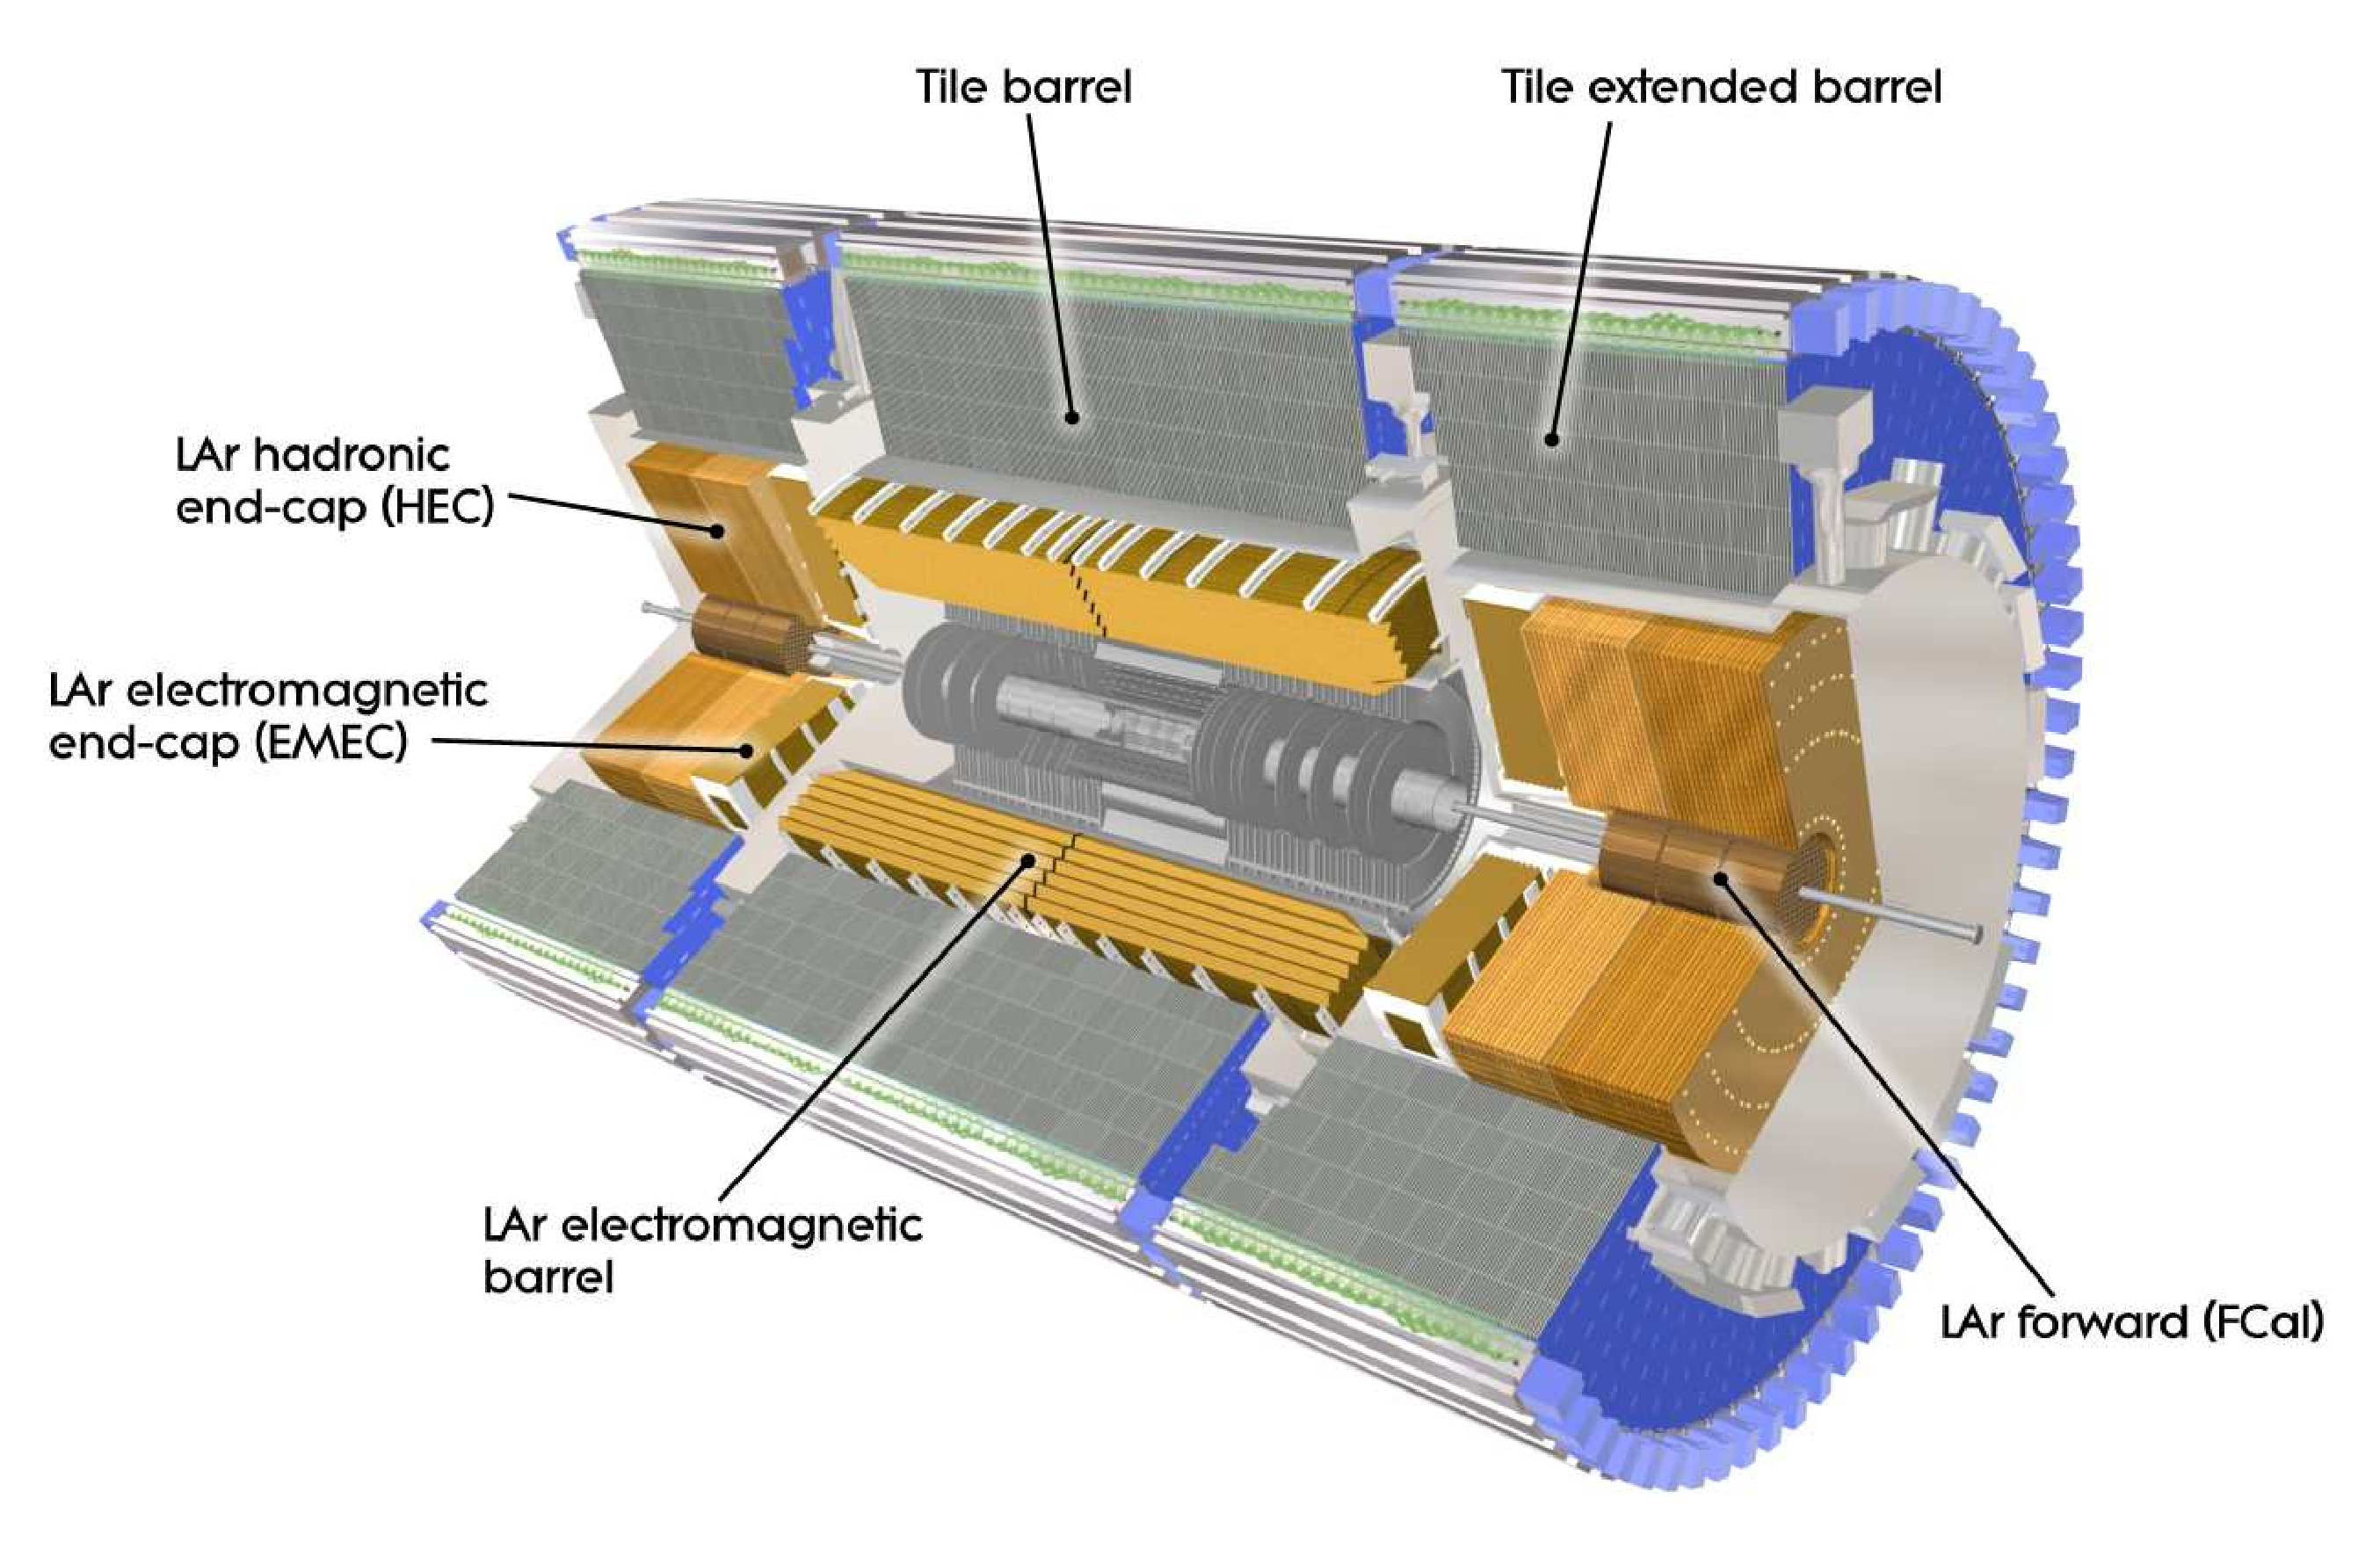
\includegraphics[width=1.0\textwidth]{LHCAtlas/Calorimeter.pdf}
\caption{Cut-away view of the ATLAS calorimeter system \cite{AtlasExperiment}.}
\label{fig:ATLASCalo}}
\end{figure}

The general structure of the \atlas calorimeter is shown in Fig.~\ref{fig:ATLASCalo}. The calorimetric system consists of a barrel ($|\eta|$ < 3.2) and two end-cap parts (3.1 < $|\eta|$  < 4.9). The central part is used for the high-precision measurements, while the end-cap part with its coarser granularity is mostly used for the jet reconstruction and  the \etmiss measurements. 

Particles, entering the calorimeter, produce a cascade of secondary particles called a particle shower. Each shower is registered by a set of smallest structures of the calorimeter (so-called cells). The distribution of cells energies differs for different types of particles and can be used for particle identification. 

In order to measure the energy of the particle properly, calorimeters must provide good containment for showers.  Since the depth of the shower, caused by the electromagnetic particle is significantly smaller than the depth of the hadronic shower, calorimeters are divided into two types: electromagnetic (EM) and hadronic. EM calorimeters are placed closer to the interaction point and have a smaller amount of the dead material, compared to the hadronic calorimeters. The depth of the calorimeter is adjusted using  the dead material, that does not produce any signal response. The full particle energy is reconstructed from the ratio between tbe amount of energy absorbed in the dead and active material.

In the central region, calorimeters are required to have high granularity for combination with ID information and a precision measurement of photons and electrons. 

\subsubsection{Electromagnetic calorimeter}
\begin{figure}[!tb]
\center{
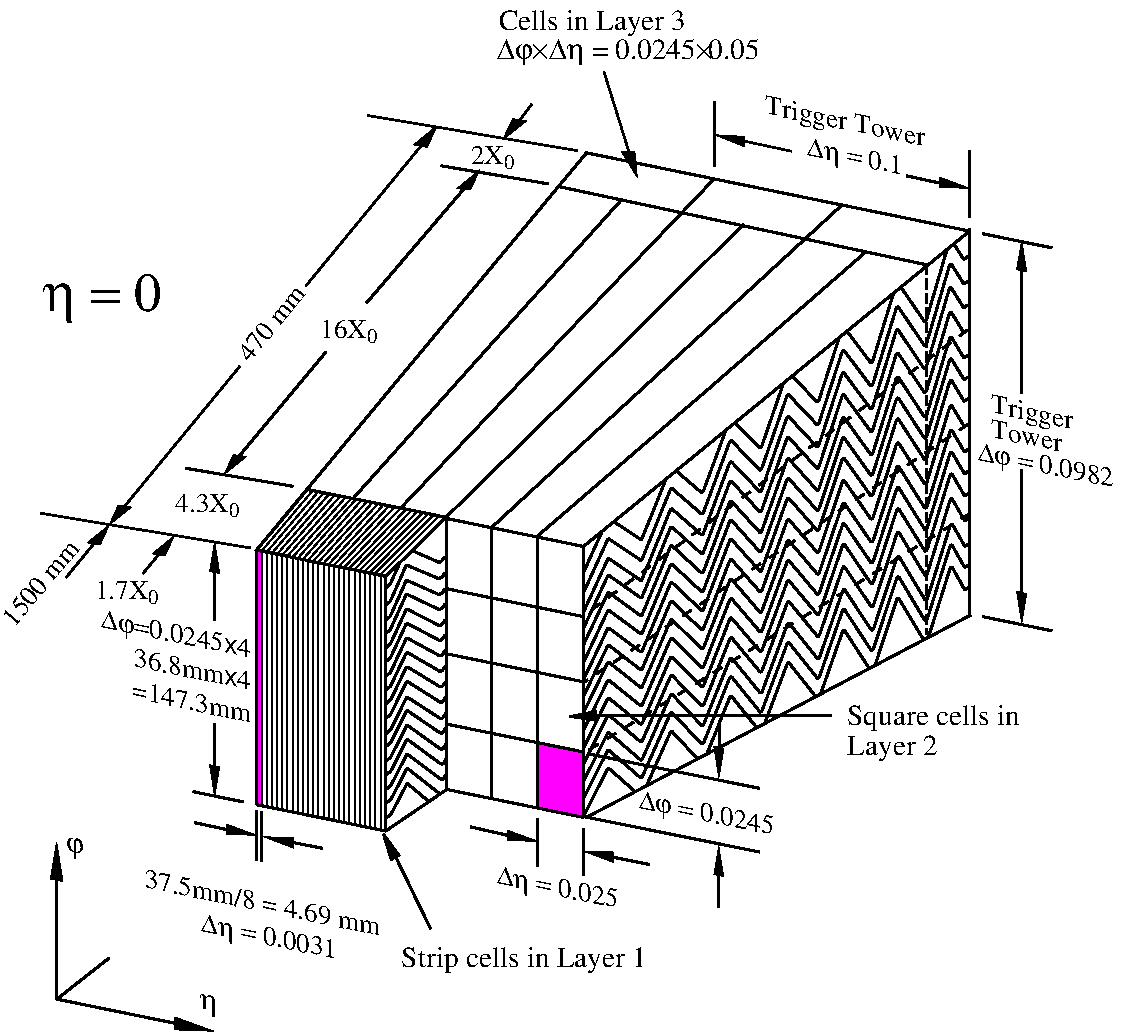
\includegraphics[width=0.7\textwidth]{LHCAtlas/BarellCalo.pdf}
\caption{The sketch of EMB module at $\eta\approx0$.  The granularity in $\eta$ and $\phi$ of each of the three layers is also shown \cite{AtlasExperiment}.}
\label{fig:ATLASCaloEM}}
\end{figure}

The main purpose of the electromagnetic calorimeter is to measure energies of electrons and photons. The shower production in EM calorimeter is mainly determined by electron-positron pairs production and photons emitting via bremsstrahlung. The EM shower starts from initial high-energy electron or photon entering the calorimeter. The EM calorimeter consists of a barrel part (EMB) and two symmetric end-caps (EMEC), that cover a range of pseudorapidity of $|\eta|<1.475$ and $1.5 < |\eta|<3.2$ respectively. The EM calorimeters have an accordion structure, as shown in Fig.~\ref{fig:ATLASCaloEM}. This geometry allows for a full coverage in the $\phi$ coordinate.
The calorimeters consist of the layers of lead/steel, interplaced with liquid argon, that acts as a sensitive material.

The EMB calorimeter consist of four sampling layers:
\begin{itemize}
\item \textbf{presampler} A single layer of LAr without dead material. It allows to correct for the energy loss in front of the calorimeter. It covers the pseudorapidity range of $|\eta|<1.8$;
\item \textbf{1st sampling} The first layer has a fine segmentation in $\eta$ with thin $\eta$ strips with size $\Delta \eta \times \Delta \phi = 0.0031 \times 0.098$. Thanks to the fine granularity this layer provides an information for $\gamma$ and $\pi^0$ separation;
\item \textbf{2nd sampling} The majority of the energy is deposited in the second sampling layer. It consists of the square cells with size $\Delta \eta \times \Delta \phi = 0.0245 \times 0.0245$;
\item \textbf{3rd sampling} Only the highest energy electrons are reaching the third layer. Size of the cells in this layer is $\Delta \eta \times \Delta \phi = 0.0245 \times 0.05$
\end{itemize}
All of the sampling layers, except for the presampler are shown in Fig.~\ref{fig:ATLASCaloEM}.

Each wheel of the EMEC calorimeter consists of 2 co-axial wheels: Inner Wheel (IW) and Outer Wheel (OW). Each endcap wheel is divided into 8 wedge-shaped modules. In the central region ($1.5<|\eta|<2.5$), the EMEC calorimeter consists of 3 layers with granularity $\Delta \eta \times \Delta \phi = 0.025 \times 0.025$. 

\subsubsection{Hadronic calorimeter}

The mechanism of hadronic shower development differs from the relevant process in EM one. The main physical processes, determining the shower development are hadron production, nuclear deexcitation and pion decays. The \atlas hadronic calorimeter consists of the central part (tile), the hadronic end-cap calorimeter (HEC) and the forward part of the hadronic calorimeter (discussed separately).

The tile calorimeter is placed right after the EMEC and covers a pseudorapidity range up to $|\eta|$=1.0 in the barrel region and 0.8 < $|\eta|$ < 1.7 in the two end-caps. It is a sampling calorimeter with steel acting as a dead material, and the scintillator ties for a sensitive material. The signal readout from the scintillator is performed using the wavelength shifting fibers.  The readout cells are built by grouping several fibers into the single photomultiplier.

The HEC calorimeter uses a liquid argon as a sensitive material and shares the same LAr cryostat with EMEC. The copper plates are acting as an absorbers. The size of the cell in HEC is $\Delta \eta \times \Delta \phi = 0.1 \times 0.1$ for $|\eta|$ < 2.5 and $\Delta \eta \times \Delta \phi = 0.2 \times 0.2$ for forward region 2.5 < $|\eta|$ < 3.2.


\subsubsection{Forward calorimeter}


\begin{figure}[!tb]
\begin{minipage}[h]{0.45\linewidth}
\center{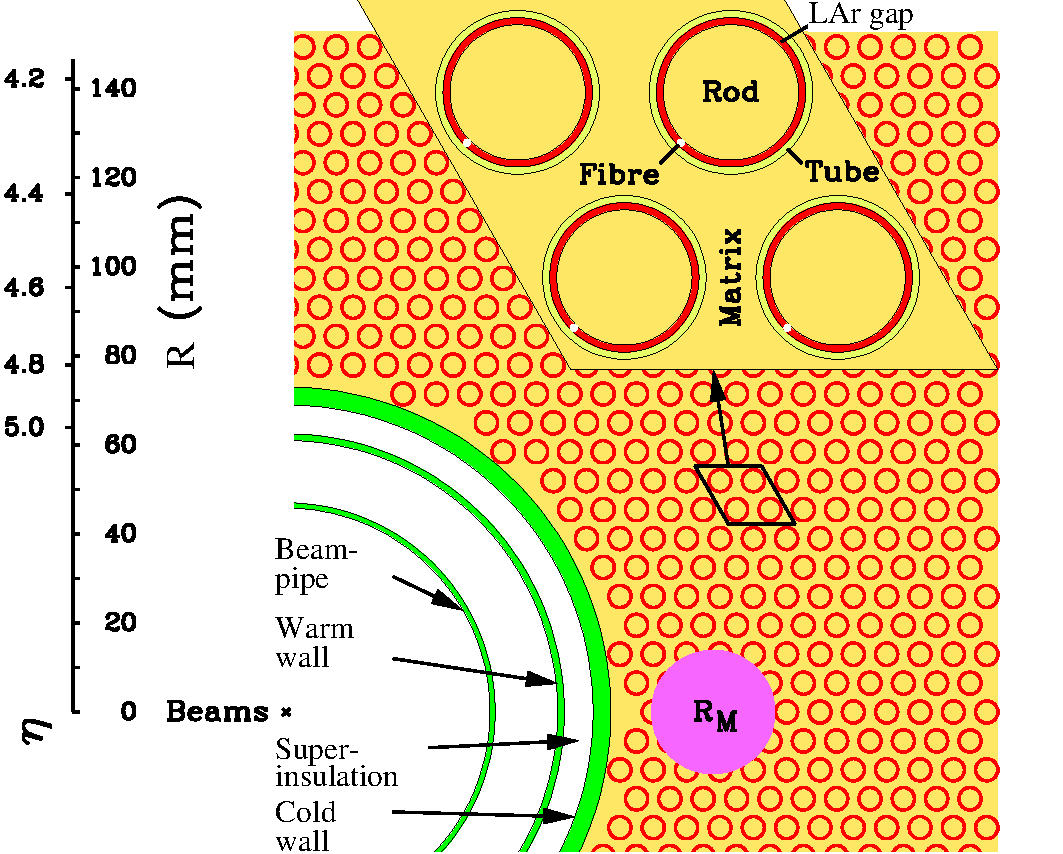
\includegraphics[width=1.\linewidth]{LHCAtlas/FCAL.pdf} }
\caption{Electrode structure of FCAL1 with the matrix of copper plates and copper tubes and rods with the LAr gap for electrodes \cite{AtlasExperiment}.}
\label{fig:FCALModel}
\end{minipage}
\hfill
\begin{minipage}[h]{0.49\linewidth}
\center{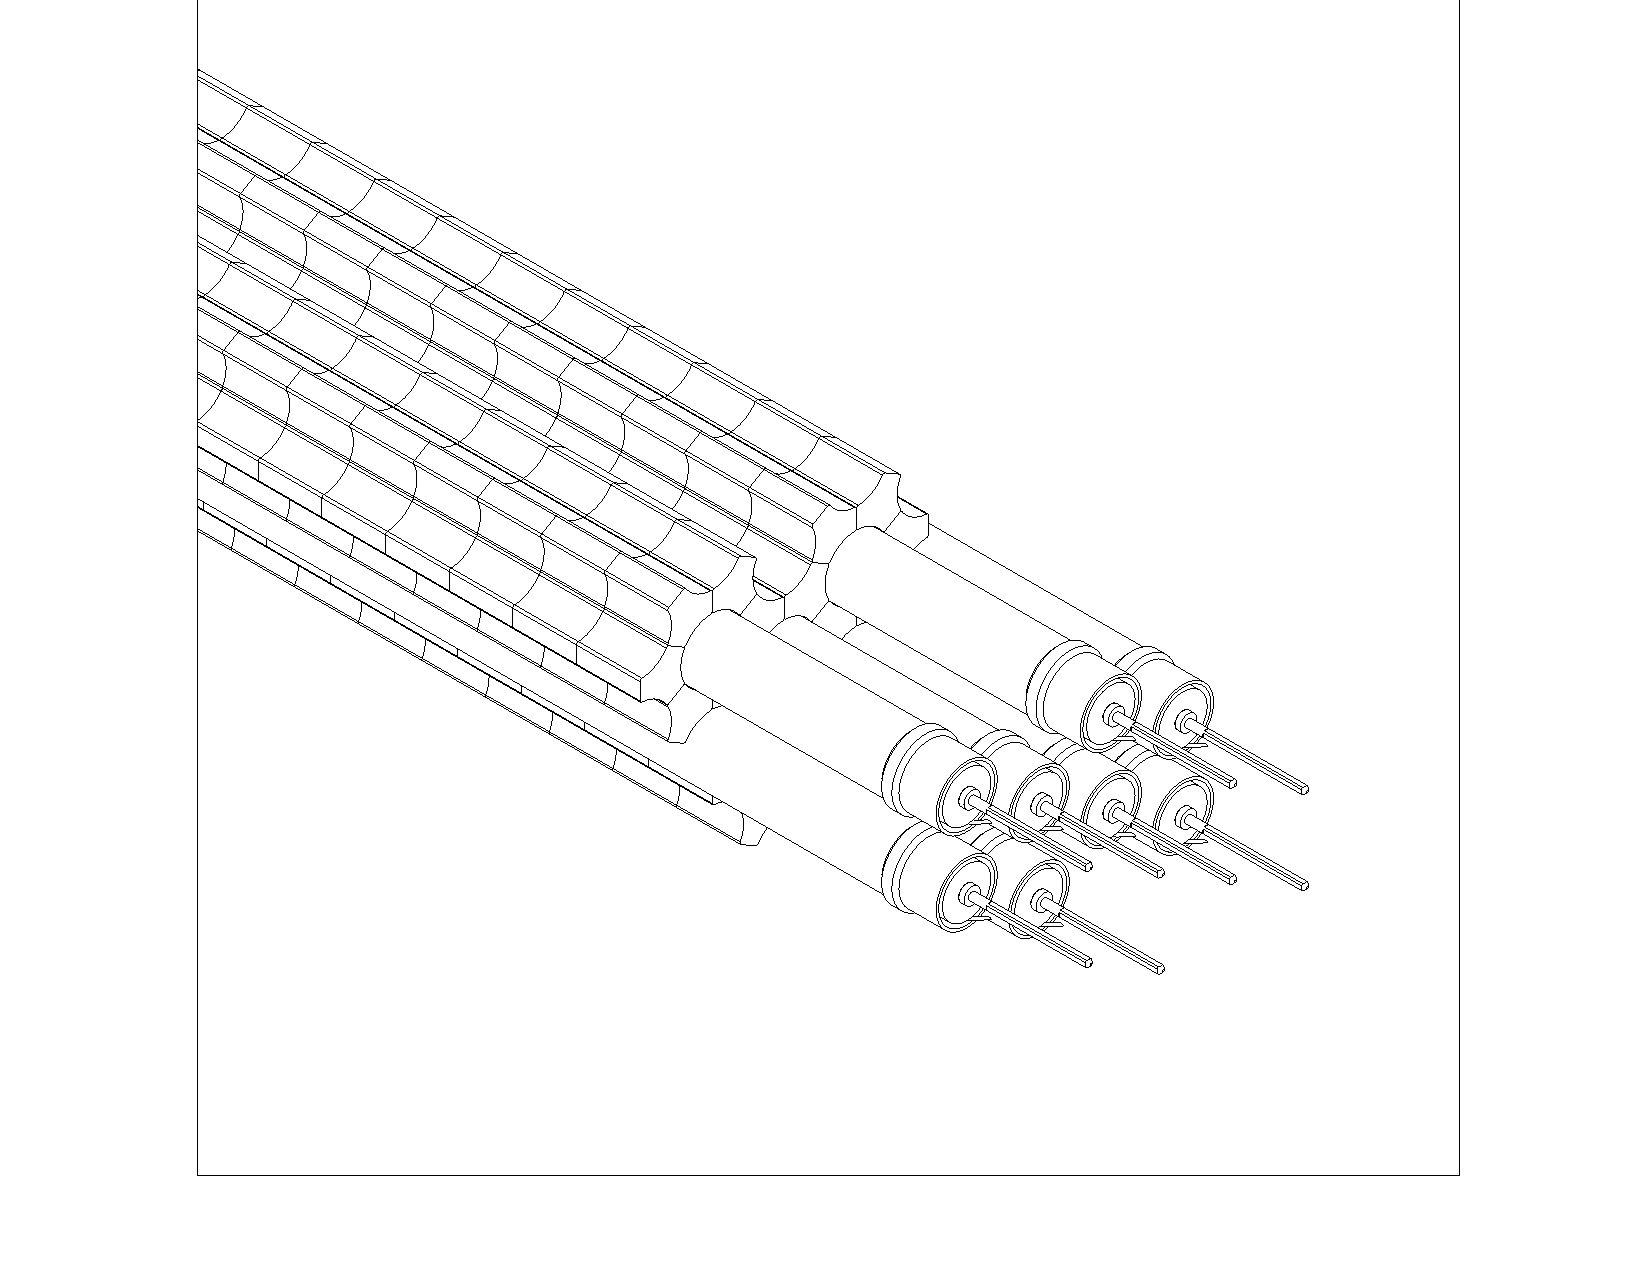
\includegraphics[width=1.\linewidth]{LHCAtlas/FCALMod.pdf}}
\caption{View of the FCAL hadronic module absorber matrix, including a set of tungsten rods and copper tubes surrounded by 1 cm long tungsten slugs\cite{AtlasExperiment}.}
\label{fig:FCAL2}
\end{minipage}
\end{figure}


The forward calorimeter (FCAL) shares the same cryostat with EMEC and covers the pseudorapidity range of  3.1 < $|\eta|$ < 4.9. It is placed 4.7 m away from the interaction point and imposed to very high particle fluxes. This motivates the choice of detector design, with a small amount of the sensitive material.  The FCAL module consists of the co-axial copper rods and anode tubes, separated by the wires around each rod. The LAr fills the gap between the rod and the anodes. The small size of the gaps allows to have a faster signal and helps to avoid signal degradation caused by distortion of the electric field in the gap. The structure of the FCAL calorimeter is shown in Fig.~\ref{fig:FCALModel}.

The FCAL is divided into 3 modules: one electromagnetic (FCAL1) and two hadronic (FCAL2 and FCAL3). Parameters of these modules are summarized in Tab.~\ref{tab:FCALParam}. In hadronic modules, a tungsten is used instead of copper, in order to keep the large absorption length. These modules are similar to the FCAL1, except for the use of tungsten rods instead of the copper rods. The space between the end-plates and tubes in FCAL2 and FCAL3 is filled with tungsten slugs, as shown in Fig.~\ref{fig:FCAL2}. The readout is formed from the group of four, six and nine electrodes for FCAL1, FCAL2 and FCAL3 respectively. The granularity of the FCAL is about $\Delta \eta \times \Delta \phi \approx 0.2 \times 0.2$.

\begin{table}[!tb]
\caption{Table of parameters for the three FCAL modules.}
\label{tab:FCALParam}
\begin{center}
\begin{tabular}{ l | c | c | c | c | c }
\hline
Module & Type & Absorber & Gap width & Number & Number \\
 & & &  ($\mu m$)  & of electrodes & of readout channels \\
\hline
\hline
FCAL1 &  electromagnetic & copper & 250 & 12 260 & 1008\\
FCAL2 &  hadronic & tungsten & 375 & 10 200 & 500\\
FCAL2 &  hadronic & tungsten & 500 & 8 224 & 254\\
\hline
\end{tabular}
\end{center}
\end{table}

\subsection{Muon Spectrometer}\label{sec:MuonSys}
The muon trajectories are  measured in the ID, however, for a high-$P_{T}$ muons, it could be difficult to make a precise determination of the charge and the momentum. The Muon Spectrometer (MS) allows to measure more precisely muon momentum and is used for the muon identification. The MS is placed in the outermost part of the \atlas detector, close to the calorimeters. The cut-off view of the MS is shown in Fig.~\ref{fig:ATLASMuon}.

The Muon Spectrometer covers the area up to $|\eta|$ = 2.7 and allows to trigger on the particles in the range $|\eta|$ < 2.4. The precision muon tracking is performed by the Monitored Drift Tubes (MDT). The MDT consist of 8 layers of the drift tubes and allow for a position resolution of 80 $\mu$m per tube (or 35 $\mu$m per chamber). In addition, in the forward region (2.0 < $|\eta|$ < 2.7), the Cathode-Strip Chambers (CSC) are used. The CSC are the multiwire proportional chambers and give a spacial resolution of 40 $\mu$m in the bending plane and 5 mm in the transverse plane.

The trigger system in the Muon Spectrometer consists of the fast Resistive Plate Chambers (RPC) and Thin Gap Chambers (TGC) located in the barrel ($|\eta|$ < 1.05) and end-cap (1.05 < $|\eta|$ < 2.4) regions respectively. 

\begin{figure}[!tb]
\center{
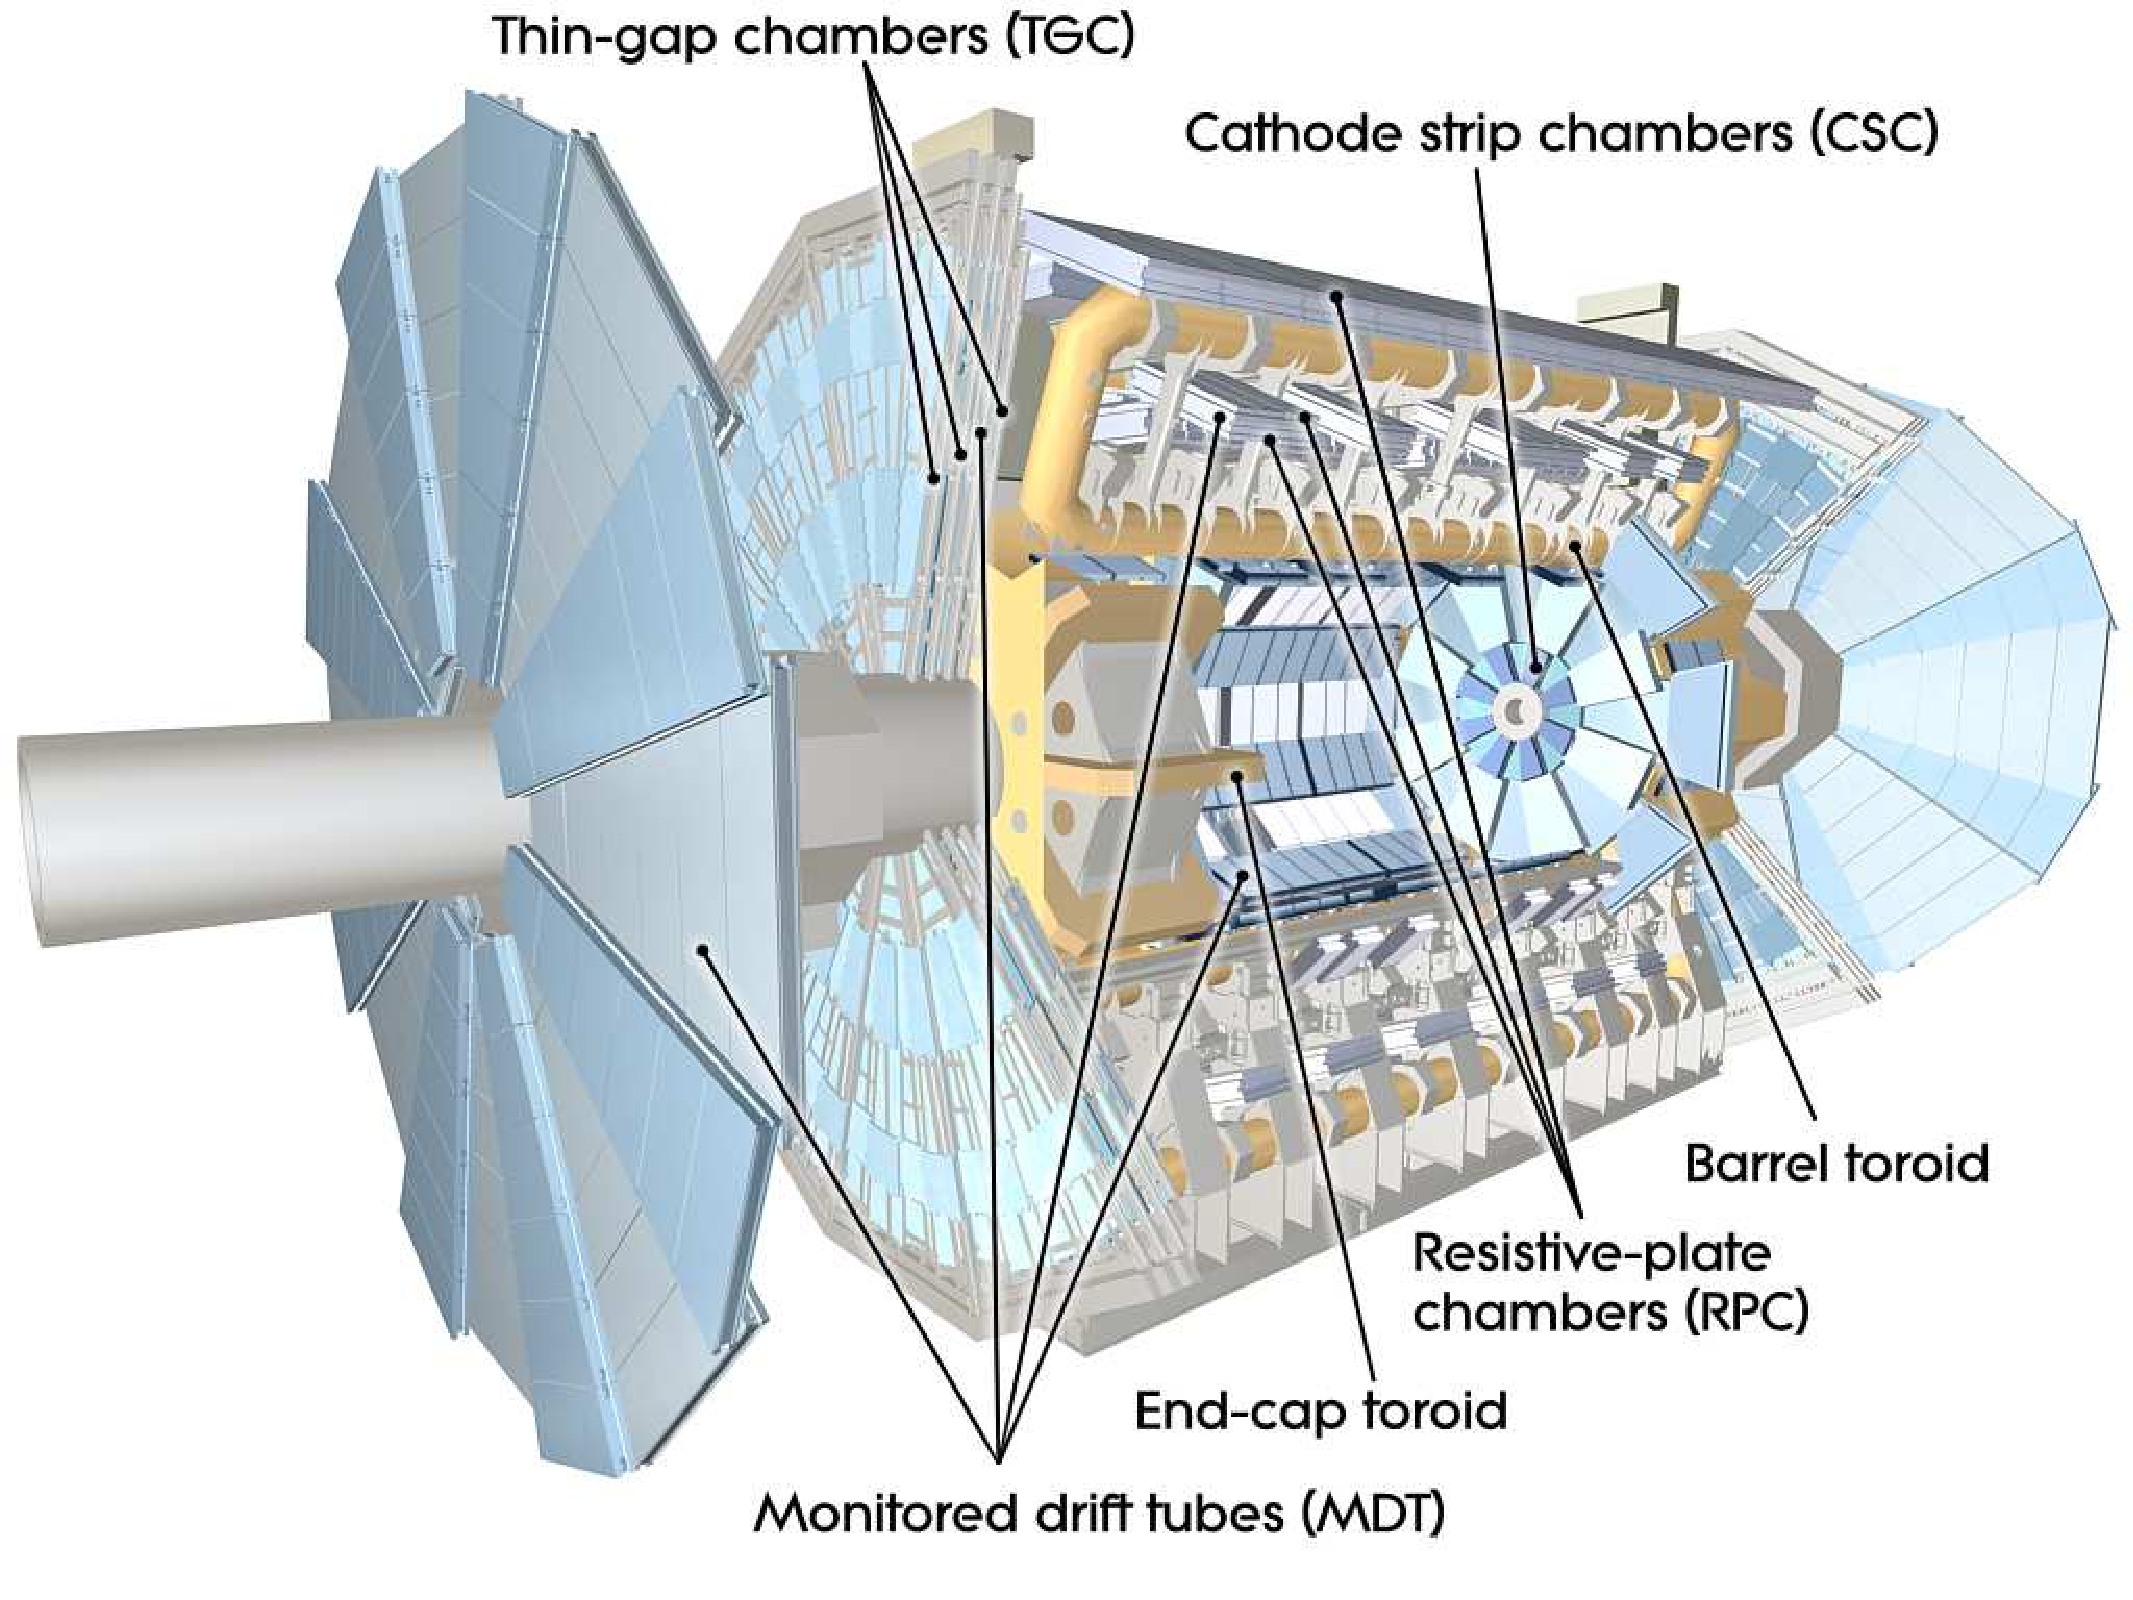
\includegraphics[width=0.8\textwidth]{LHCAtlas/MuonSystem.pdf}
\caption{Cut-away view of the ATLAS muon spectrometer \cite{AtlasExperiment}.}
\label{fig:ATLASMuon}}
\end{figure}

\subsection{Trigger system}
The trigger system is used for reducing the information stored while leaving "interesting" events untouched. The trigger system in \atlas is divided into 3 steps:
\begin{description}
\item[Level-1] The first level trigger has a high operation speed and it uses reduced-granularity information from Resistive Plate Chambers (RPC) and Thin-Gap Chambers (TGC) and calorimeter systems. It searches for leptonic and hadronic signatures (or large total transverse energy) in the detector. This trigger allows to reduce a rate, that can be handled by a readout electronics ($\sim$ 75 kHz);
\item[Level-2] The second-level \atlas trigger can analyze in more details Regions-of-Interest (RoI's) identified by Level-1 trigger. It uses an information on RoI's, such as energy and a position of clusters to further reduce the rate of events. The output Level-2 event rate is below 3.5 kHz;
\item[High-Level Trigger (HLT)] The final level trigger selection is performed offline on a large scale computing farm. CPU cores analyze a full information from detectors to refine the trigger selections. The additional information from tracking allows to improve particle identification and distinguish electrons and photons. About 200 events per second are left after the HLT selection criteria and are transmitted further to the permanent storage.
\end{description}

\section{Luminosity measurement}

One of the main components, characterizing the collider is its instantaneous luminosity $\lumi$, that is defined as a proportional factor between the cross section for a given process $\sigma$ and the number of interactions per second $\frac{dR}{dt}$:
\begin{equation}
\frac{dR}{dt}= \lumi \times \sigma (cm^{-2}s^{-1}).
\end{equation}

At the LHC the instantaneous luminosity can be calculated as:
\begin{equation}
\lumi = \frac{N_p^2 N_b f_{\textrm{rev}}}{4\pi  \sigma_x \sigma_y}F , 
\end{equation}
where $N_{p}$ is the number of protons per beam, $N_b$ - number of bunches, $f_{\textrm{rev}}$ is the revolution frequency, $\sigma_x$ and $\sigma_y$ are the horizontal and vertical beam profile widths. The factor $F$ comes from the beam crossing angle. In 2012, at $\sqrt{s}=$8 TeV, the LHC reached an instantaneous luminosity of $7.7\times10^{33}\, [cm^{-2}s^{-1}]$. 

Instantaneous luminosity can also be measured from the interaction rate $\mu_{vis}$ in a detector of some process as:
\begin{equation}
\lumi = \frac{\mu_{vis}N_b f_{rev}}{\sigma_{vis}},
\end{equation}
where $\sigma_{vis}$ is the visible interaction cross section and $\mu_{vis}$ is the visible in the detector interaction rate.

The \atlas experiment uses several detectors to measure the instantaneous luminosity. The Beam Condition Monitors (BCM) are used to monitor beam parameters close to the interaction point and allow to measure bunch intensities. In the forward region, a special detector for a luminosity measurements is placed: the LUCID (LUminosity measurement using Cerenkov Integrating Detector). The beam profile and the visible interaction cross section $\sigma_{vis}$ are measured during so-called van-der-Meer scans \cite{vanderMeer}. 
